\documentclass[a4paper,12pt,titlepage]{scrartcl}
\usepackage[utf8]{inputenc}
\usepackage{graphicx}
\usepackage{listings}
\usepackage{xcolor}
\usepackage{titlepic}
\usepackage{pdfpages}

\lstset{
    frame=tb, % draw a frame at the top and bottom of the code block
    tabsize=4, % tab space width
    showstringspaces=false, % don't mark spaces in strings
    numbers=left, % display line numbers on the left
    commentstyle=\color{green}, % comment color
    keywordstyle=\color{blue}, % keyword color
    stringstyle=\color{red} % string color
}


\title{NVS Projekt2: Remote Method Invocation System 43}
\author{Ralf Kühmayer, 13, 5BHIF}
\date{April 2021}


\begin{document}


\maketitle

\newpage

\tableofcontents

\newpage


\section{Aufgabenstellung}
Impelentierung eines Remote Method Invocation Systems basierend auf asio. Der Server und der Client müssen mit spdlog Logdateien anlegen können und JSON soll verwendet werden, entweder für die Kommunikation oder für die Konfiguration.

\section{Remote Method Invocation}

\subsection{Theorie}

\subsection{Umsetzung}
In diesem Programm wurden drei Objekte angelegt. Welche dem Server und dem Client bekannt sein müssen. Diese Objekte werden zwischen Server und Client synchronisiert und der Client kann Funktionen der Objekte am Server aufrufen. Zu diesen Objekten gehört der Car\_Builder, welcher als Grundobjekt dient. Mit diesem Car\_Builder, kann man ein Objekt, ein Car, erzeugen, welches im weiteren Verlauf an den Car\_Calculator übergeben wird. Das Car an sich kann nur angesehen werden und es gibt keine Möglichkeit, es zu verändern. Der Car\_Calculator benötigt dann noch ein paar zusätzliche Infos und kann, basierend auf diesen Informationen dann zwei Berechnungen ausführen. Diese Berechnungen wird der Client am Server durchführen. Um ein paar Attribute des Cars besser darstellen zu können, gibt es drei Enums welche die jeweiligen Typen besser benennen. Die drei Grundobjekte werden dann am Server in dem Object\_Storage verwaltet. Dieser führt die vom Client gesendeten Operationen aus und überprüft, ob alle Bedingungen gegeben sind, gegebenenfalls gibt er das erwartete Ergebnis oder eine Fehlermeldung zurück. Damit die Kommunikation über Streams in assio mit Protobuff funktioniert, gibt es den Namespace message\_utility, welcher dafür sorgt, dass die zu String serialisierten Protobuff Objekte über einen Stream übertragen werden können. Dies ist notwendig, da in den serialisierten Protobuff Objekte \textbackslash n vorkommt, welches zu auslesen des Streams am Server führen würde. Daher werden die serialisierten Protobuff Objekt mit der Methode to\_ascii codiert und dann beim Empfänger wieder mit der Methode from\_ascii decodiert.Damit der Benutzer über den Client mit dem Server kommunizieren kann und Objekte erstellen und Methoden ausführen kann, gibt es das Repl, welches die Eingaben des Benutzers liest, diese validiert und die dem entsprechend Methoden, Änderungen, Ausgaben oder Kommunikationen mit dem Server vornimmt. Um generelle Konfigurationen auf dem Server und auf dem Client vor nehmen zu können, gibt es den Namespace config. In diesem Namespace liegen zwei Structs und mehrere Konfigurationsfunktionen. Eines der beiden Structs ist das Server Struct. In diesem Struct werden die Informationen bezüglich der IP-Adresse, des Portes und ob der Server vom Client geschlossen werden darf, gespeichert. Die Information über die IP-Adresse und des Portes ist für den Client wichtig, damit er eine Verbindung aufbauen kann. Die Information über den Port und ob der Server vom Client geschlossen werden darf, hingegen ist für den Server wichtig. Das zweite Struct, Log\_Settings, legt sowohl am Client als auch am Server die Konfiguration des Loggers fest und gibt diese in einem lesbaren Format aus. Die zusätzlichen Funktionen in dem config Namespace dienen der allgemeinen Konfiguration. Sie erlaben es sowohl den Client als auch den Server über eine JSON- oder eine TOML-Datei zu konfigurieren und validieren diese beiden Dateiarten auch. Des Weiteren gibt es noch die Funktion, den Server zu starten, welche benötigt wird, wenn der Client angibt, dass er den Server mit starten will.

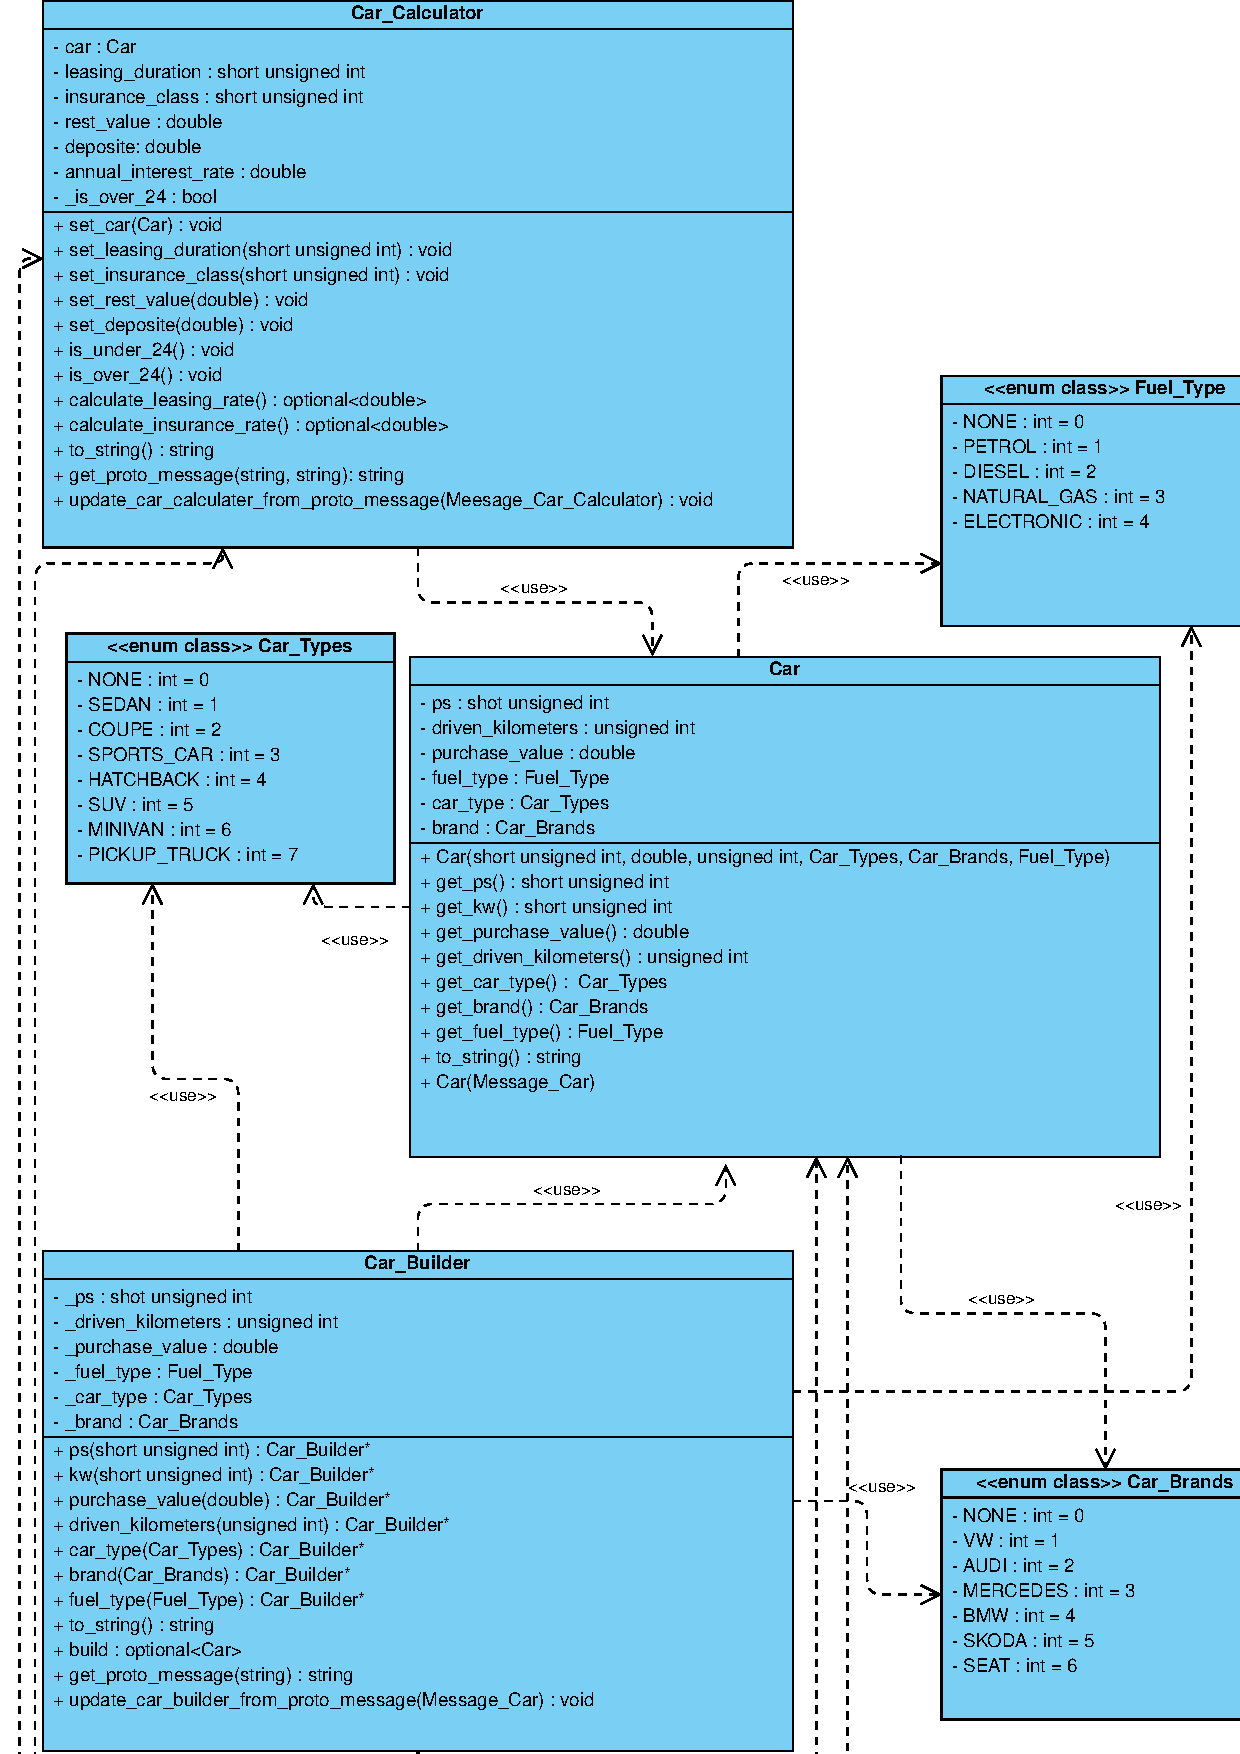
\includepdf[pages={1-},scale=0.9]{test.pdf}
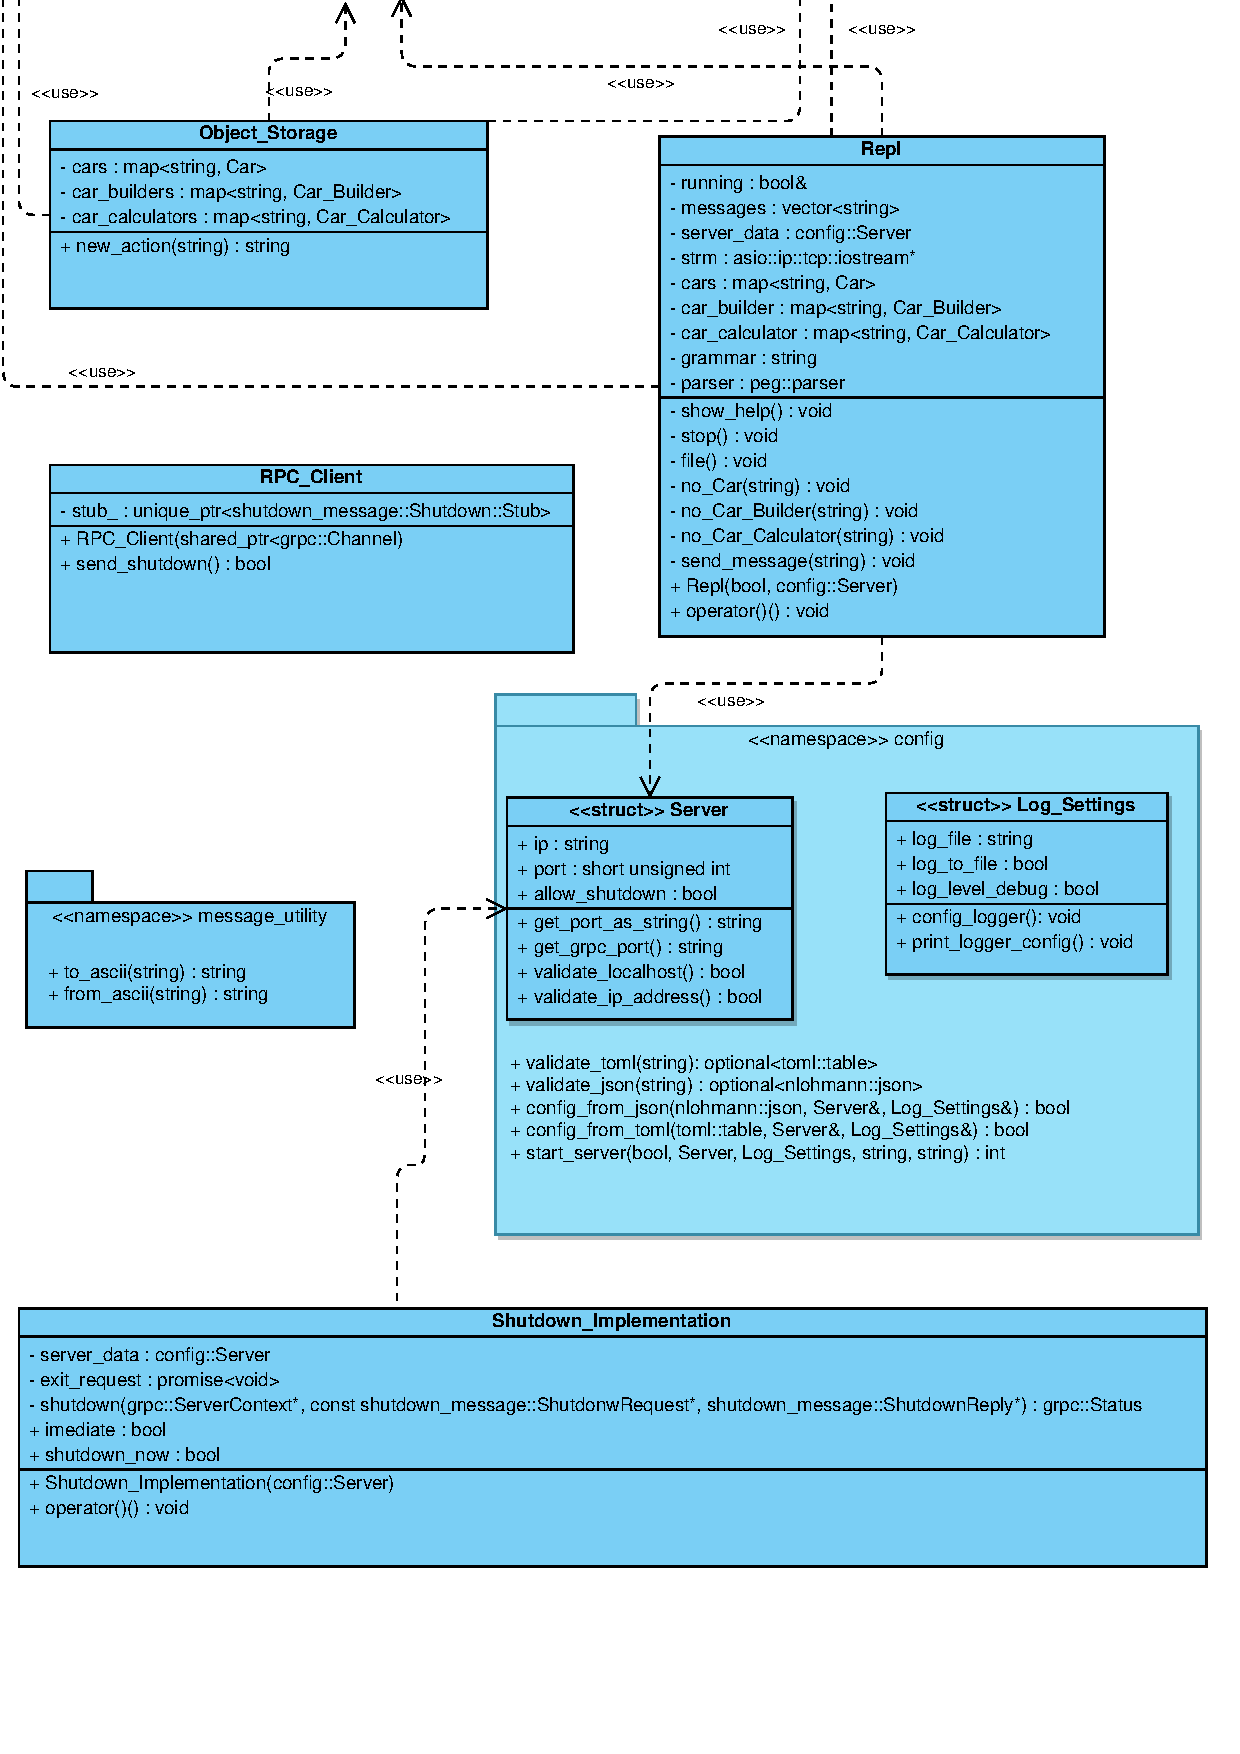
\includepdf[pages={1-},scale=0.9]{test2.pdf}
\subsection{Bedienung} %Sourcecode examples


\section{Programm}

\subsection{Parameter}
Bei beiden Programmen kann man die Parameter in Logging-Parameter, Connection-Parameter und Konfiguration-Parameter einteilen. Wobei diese Parameter bis auf einige Spezifische auf dem Server und dem Client gleich sind.

\paragraph{Logging-Parameter}

\paragraph{-l,\texttt{-{}-}log-to-file}
Mit diesem Parameter kann der Benutzer das Logging in eine externe Datei aktivieren. Wird nur dieser Parameter angegeben, ist das Log-Level per Default auf Info gestellt und der Logger erstellt eine Datei in einem Unterverzeichnis log mit dem Namen server.log oder client.log.

\paragraph{-d,\texttt{-{}-}log-level-debug}
Will man mehr Daten sehen, um z. B. einen Fehler im Programm zu finden. Kann man mit diesem Parameter das Log-Level auf Debug setzen. Dadurch werden mehrere Informationen in die Log-Datei geschrieben. Dieser Parameter kann nur angegeben werden, wenn auch der Parameter "-l,\texttt{-{}-}log-to-file" angegeben wurde.

\paragraph{\texttt{-{}-}log-file $<Dateipfad>$}
Soll die Log-Datei in einem bestimmten Verzeichnis mit einem bestimmten Namen platziert werden, muss dieser Parameter und ein Dateipfad mit Dateinamen angegeben werden. Existiert diese Datei bereits, wird sie überschrieben. Wenn diese Datei größer als 10 MB wird, legt der Logger bis zu drei Dateien an. Sind alle drei Daten größer als 10 MB, wird begonnen, die erste zu überschreiben. Dieser Parameter kann nur angegeben werden, wenn auch der Parameter "-l,\texttt{-{}-}log-to-file" angegeben wurde.

\paragraph{Connection-Parameter}

\paragraph{-p,\texttt{-{}-}port $<positive \: ganze \: Zahl>$}
Mit diesem Parameter wird für den Server der Port angegeben, auf welchem er auf Anfragen hören soll. Für den Client gibt dieser Parameter an, auf welchem Port er die Anfragen schicken soll. Es wird nicht nur der angegebene Port, sondern auch der nächsthöhere Port verwendet. Wird dieser Parameter nicht angegeben, wird der Defaultport verwendet. Dieser Defaultport ist Port 1112.

\paragraph{Client: -s,\texttt{-{}-}server-ip $<Hostname \: oder \: IP-Adresse>$}
Dieser Parameter ist nur für den Client bestimmt, da der Server die IP-Adresse des Gerätes, auf welchem er gestartet wurde, annimmt. Wird an diesem Parameter eine IP-Adresse übergeben, dann wird sie validiert, ob sie allen Richtlinien einer IP-Adresse entspricht. Wird dieser Parameter nicht angegeben, wird der Client mit Localhost als IP-Adresse gestartet.

\paragraph{Konfiguration-Parameter}

\paragraph{-j, \texttt{-{}-}config-file-json $<Dateipfad>$}
Mit dem Parameter -j oder \texttt{-{}-}config-file-json und dem Pfad zu der Konfigurationsdatei kann angegeben werden, dass das Programm mit einer JSON-Datei konfiguriert werden soll. Wird dieser Parameter angegeben, werden alle Parameter überschrieben, welche in der Konfigurationsdatei konfiguriert werden.

\paragraph{-t, \texttt{-{}-}config-file-toml $<Dateipfad>$}
Mit dem Parameter -t oder \texttt{-{}-}config-file-toml und dem Pfad zu der Konfigurationsdatei kann angegeben werden, dass das Programm mit einer TOML-Datei konfiguriert werden soll. Wird dieser Parameter angegeben, werden alle Parameter überschrieben, welche in der Konfigurationsdatei konfiguriert werden.


\paragraph{Spezifische Parameter}


\paragraph{Client: \texttt{-{}-}start-server}
Mit diesem Parameter kann man angeben, dass der gestartete Client auch gleich einen Server startet. Dieser gestartete Server wird auch geschlossen, wenn der Client geschlossen wird. Wird dieser Parameter angegeben, erweitert sich die Validierung der IP-Adresse darauf, dass nur Localhost IP-Adressen valide sind. Das ist daher zu erklären, da, wenn man den Server auf seinem eigenen PC startet, dieser immer nur mit Localhost als IP-Adresse angesprochen werden kann.


\paragraph{Server: -e,\texttt{-{}-}enable-shutdown}
Mit diesem Parameter kann man angeben, dass der gestartete Server sich durch einen grpc Aufruf des Clients schließen lassen kann. Dies wird vor allem benötigt, da der Client den Server mit starten kann und dann diesen auch schließen können muss.


\subsection{Server}
Beim Starten des Servers werden zuerst alle Parameter auf ihre Richtigkeit überprüft und die Konfiguration basierend auf diesen Einstellungen vorgenommen. Wurde alles richtig konfiguriert, wird der Endpunkt des Servers erstellt. An diesen Endpunkt wird der eingetragenen Port übergeben. Ist dieser Port schon belegt, wirft der Endpunkt einen Error und das Programm beendet sich. Ist der Port jedoch nicht belegt, wird auf diesem Port auf anfragen gewartet. Dieses warten auf Anfragen passiert in einem eigenen Thread, sodass auch ein grpc-Server gestartet werden kann. Dieser Server überprüft auch zuerst, ob sein angegebener Port noch frei ist. Ist bei keinem der beiden Endpunkte ein Fehler aufgetreten, wird eine Nachricht ausgegeben, dass der Server gestartet ist. Jetzt wartet der Server auf Anfragen. Erhält der Server eine Anfrage, erstellt er für diese einen eigenen Thread und erstellt einen eigenen Object-Storage. Dieser überprüft jede Anfrage und sendet je nach dem eine Fehlermeldung oder ein Objekt zurück. Schließt der Client die Verbindung, wird der Object-Storage gelöscht und der Thread beendet sich. Der Server läuft solange weiter, bis er von einem Client oder durch eine Benutzereingabe das Zeichen bekommt, sich zu beenden. Erhält er dieses Zeichen, schließt er alle Verbindungen und beendet das Programm.


\subsection{Client}
Beim Starten des Clients werden zuerst alle Parameter auf ihre Richtigkeit überprüft und die Konfiguration basierend auf diesen Einstellungen vorgenommen. Wurde alles richtig konfiguriert, startet der CLient das Repl. Beim Start des Repls wird überprüft ob sich der CLient zu dem Server verbinden kann. Kann keine Verbindung aufgebaut werden, schließt sich der Client. Kann eine Verbindung aufgebaut werden, werden die Benutzereingaben überprüft und für jeden validen Befehl, eine Funktion ausgeführt. Manche dieser Funktionen haben zur Folge, dass Objekte zwischen dem Server und dem Client synchronisiert werden müssen. Wird bei so einem Befehl festgestellt, dass der Server nicht mehr erreichbar ist, wird dem Benutzer die Option gegeben, das Programm zu beenden oder es erneut zu versuchen. Ist der Server jedoch erreichbar werden die Objekte synchronisiert. Es gibt auch Befehle, welche es erfordern, dass der Server eine Methode ausführt und dem Client das Ergebnisse zurück gibt. Will der Benutzer das Programm beenden, muss er den Endbefehl eingeben. Die Verbindung zum  Server wird geschlossen und falls der Benutzer den Server mit dem Client mit gestartet hat, wird auch der Server geschlossen.

\end{document}